%% ==========================================================================
%% Self-Healing Routing on a Real Urban Road Network
%% JOURNAL-LENGTH version (IEEEtran journal class, ~12 pp).
%% NOT the default document: the conference paper is main.tex.
%% Set the main document explicitly if you want to build this one.
%%
%% BUILD: this repository has no LaTeX toolchain. Upload this directory to
%% Overleaf (or run latexmk locally) -- see README.md in this folder.
%% ==========================================================================
\documentclass[journal]{IEEEtran}

\usepackage[T1]{fontenc}
\usepackage[utf8]{inputenc}
\usepackage{graphicx}
\usepackage{amsmath}
\usepackage{amssymb}
\usepackage{booktabs}
\usepackage{multirow}
\usepackage{url}
\usepackage{xcolor}

% IEEEtran prefers \eqref-free math; keep equations simple.
\graphicspath{{figures/}{../../figures/ieee/}}

\begin{document}

\title{Self-Healing Routing on a Real Road Network:\\
Ant Colony Optimization and Physarum versus\\
Classical Shortest-Path Algorithms}

% \linebreakand is provided by IEEEtran in conference mode only; this
% guard lets the identical author block compile in journal mode too.
\providecommand{\linebreakand}{\and}
\author{
\IEEEauthorblockN{K Karthik Pai}
\IEEEauthorblockA{\textit{Dept. of Computer Science and Engineering} \\
\textit{RV College of Engineering}\\
Bengaluru, India \\
1RV25CS076}
\and
\IEEEauthorblockN{Manas Saxena}
\IEEEauthorblockA{\textit{Dept. of Computer Science and Engineering} \\
\textit{RV College of Engineering}\\
Bengaluru, India \\
1RV25CS096}
\linebreakand
\IEEEauthorblockN{Kushal Gowda S}
\IEEEauthorblockA{\textit{Dept. of Computer Science and Engineering} \\
\textit{RV College of Engineering}\\
Bengaluru, India \\
1RV25CS090}
\and
\IEEEauthorblockN{N Litheesh}
\IEEEauthorblockA{\textit{Dept. of Computer Science and Engineering} \\
\textit{RV College of Engineering}\\
Bengaluru, India \\
1RV25CS107}
\linebreakand
\IEEEauthorblockN{Prof. Nithyashree G D}
\IEEEauthorblockA{\textit{Dept. of Computer Science and Engineering} \\
\textit{RV College of Engineering}\\
Bengaluru, India \\
Faculty Mentor}
}

\maketitle

\begin{abstract}
Bio-inspired routing methods are often proposed as \emph{self-healing}:
after a road closure they are said to adapt from their retained internal
state rather than recompute from scratch. That claim is usually evaluated on
synthetic, undirected graphs without congestion, and almost never by
measuring recovery itself. We benchmark Dijkstra/A*, a MAX--MIN Ant System,
and a Physarum polycephalum tube-reinforcement model on the real road
network of central Bengaluru (2{,}856 nodes, 7{,}015 directed edges) under
congestion generated by the SUMO microsimulator, across seven closure
scenarios, two demand levels, and warm- versus cold-start recovery:
5{,}520 runs in a fully paired design.
We report three findings. First, path-extraction provenance dominates any
naive reading of Physarum's accuracy: pooled, the model matches the optimal
route on 90\% of undisrupted pairs, but using only its own maximum-flux
extraction the figure is 23.3\%, and on warm recoveries it returns the
Dijkstra fallback's path on 66.8\% of cells. Second, warm starting is a
genuine trade rather than a free lunch: it cuts recovery by 2.97$\times$ in
iterations and 6.87$\times$ in wall-clock (paired, $n=358$,
$p<10^{-51}$), with 48.3\% of warm recoveries converging in a single
iteration where cold start never does, yet it measurably degrades the
reported path ($p=4.3\times10^{-7}$). Third, the maximum-flux walk succeeds
\emph{less} often as the conductivity field converges while producing much
better paths when it does succeed, so completion and quality move in
opposite directions. We also show that the sign of the congestion effect on
ACO is a property of the congestion model, not of the algorithm. We argue
that the directed, sparse structure of a real road network --- mean
out-degree 2.46, pervasive one-way streets --- is what exposes these
effects, and that they are structurally unreachable on the complete and
near-complete undirected graphs used in prior evaluations.
\end{abstract}

\begin{IEEEkeywords}
Bio-inspired routing, ant colony optimization, Physarum polycephalum,
shortest path, network resilience, traffic simulation, benchmarking.
\end{IEEEkeywords}

\section{Introduction}

A city road network is not static. Signals, incidents, construction and
closures change the cost of travel continuously, and a routing method that is
optimal on a frozen snapshot may be worthless if it has to recompute from
nothing every time the network changes. This observation motivates a large
literature on \emph{bio-inspired} routing, in which ant colony optimization
(ACO)~\cite{dorigo1996ant,stutzle2000maxmin} and models of the slime mould
\emph{Physarum polycephalum}~\cite{nakagaki2000maze,tero2007mathematical}
maintain an internal state (a pheromone field, a field of tube
conductivities) that is claimed to let them \emph{adapt} to a change
rather than restart.

The claim is attractive and it is rarely measured. Evaluations of these
methods overwhelmingly use synthetic graphs, report accuracy on an
undisrupted shortest-path problem, and treat the adaptive machinery as
self-evidently useful. Three gaps follow. Test graphs are typically
undirected and dense, so they lack the structure (one-way streets, low out-degree, cul-de-sacs)
that makes real road routing hard. Congestion is
usually absent, so the edge weights that the adaptation is supposed to track
never move. And recovery after a disruption, the very behaviour that
justifies the adaptive state, is seldom the measured quantity.

This paper closes those gaps for one city. We benchmark classical Dijkstra and
A*~\cite{dijkstra1959note,hart1968formal}, a MAX--MIN Ant System (MMAS), and
a Tero-style Physarum conductivity model on the real road network of central Bengaluru under congestion generated by
the SUMO microsimulator~\cite{lopez2018microscopic}, and we measure recovery
from seven classes of road closure under both warm start (retained internal
state) and cold start (state reset). The design is fully paired: every
algorithm sees identical origin--destination pairs, identical closures and
identical traffic, and all quality figures are expressed against a Dijkstra
optimum computed on the same weighted graph.

\subsection{Contributions}

\textbf{1) Path extraction, not the model, decides what a Physarum result
means.} The conductivity model does not emit a route; a separate extraction
step does. We instrument that step and find that Physarum's apparent
competence is largely attributable to its fallback. Pooled over all
extraction methods it matches the optimal route on 90.0\% of undisrupted
pairs, reproducing the accuracy reported in the literature; restricted to its
own maximum-flux walk the figure is 23.3\%. The median stretch is exactly
1.000 inside \emph{every} provenance class, so a pooled number cannot
distinguish ``the model found the optimum'' from ``the fallback returned
Dijkstra's answer''. On warm recoveries the effect is starker still: the
conductivity threshold subgraph never connects origin to destination, and the
model reports plain Dijkstra's path on 66.8\% of cells. We therefore report
Physarum as two labelled series throughout and never pool them.

\textbf{2) Warm starting buys speed and charges for it in quality.}
Retaining the conductivity field across a closure reduces recovery by
2.97$\times$ in iterations and 6.87$\times$ in wall-clock, paired on
identical cells ($n=358$, $p=3.2\times10^{-59}$ and
$9.0\times10^{-52}$). The distribution is bimodal rather than merely
shifted: 48.3\% of warm recoveries converge in exactly one iteration, which cold start never achieves; its minimum is 73. Per-iteration cost is
unchanged (0.051\,s versus 0.054\,s), which is what establishes that the
saving is adaptation and not cheaper arithmetic. Against this, warm start is
significantly \emph{worse} on the reported post-disruption path
($p=4.3\times10^{-7}$). Reporting only the speed-up, as the self-healing
framing invites, would describe half of the effect.

\textbf{3) Adaptation improves extraction quality while reducing its
reliability.} Against a zero-adaptation control (the same pressure solve on a uniform
conductivity field, containing none of the Tero dynamics), the converged
field completes a walk \emph{less} often (43.3\% versus 56.7\%)
and yet produces far better routes when it does (median stretch 1.006 versus
1.437; exact match 46.2\% versus 5.9\% of completions). Completion and
quality move in opposite directions, so either measured alone misleads. This
also explains the discrepancy with prior theory: a near-uniform flux field is
easy to walk precisely because it is uninformative.

\textbf{4) The sign of the congestion effect belongs to the congestion
model.} Under an analytic BPR volume-delay function congestion \emph{helps}
ACO; under SUMO microsimulation on the same network it \emph{hurts} it
(within-10\% rate 81.3\% light versus 58.0\% heavy, paired $p=0.036$). Any
claim about behaviour ``under congestion'' that does not name its congestion
model is underdetermined.

Throughout we report what the methods lose as well as what they gain.
Dijkstra recomputes an exact route in a single iteration and roughly 31\,ms,
and no bio-inspired method here approaches that; the defensible quantities
are iterations-to-adapt and post-disruption path quality, which is the
speed-versus-quality trade this paper measures.

\section{Related Work}

\subsection{Physarum models of shortest path}

The slime mould \emph{Physarum polycephalum} connects food sources through a
tube network that thickens where flux is high and atrophies where it is
low, and it famously resolves a maze into the shortest connecting
path~\cite{nakagaki2000maze}. Tero et al.\ formalised this as a system of
adapting conductivities driven by a Poiseuille-flow pressure
solve~\cite{tero2007mathematical}; the same group later used it to produce
networks comparable to the Tokyo rail system~\cite{tero2010rules}. Bonifaci
et al.\ proved that the continuous dynamics converge to the shortest path,
for \emph{undirected} graphs~\cite{bonifaci2012physarum}. We implement the
canonical Tero model, with the simpler Bonifaci adaptation rule available as
a configuration switch. Awad et al.\ survey the wider family of
Physarum-inspired applications~\cite{awad2022survey}.

The directedness restriction is explicit in the literature rather than
incidental. Zhang et al.\ note that the model is designed only for
undirected networks and propose a directed formulation based on analog
circuit analysis~\cite{zhang2014directed}. We do \emph{not} implement that
variant; the behaviour we report for the canonical model on a directed
network should therefore be read as a measurement of an acknowledged
limitation, not as the discovery of a defect.

\subsection{The prior three-way comparison}

The combination of Physarum, ACO and Dijkstra in one study is not new.
Zhang et al.\ benchmark exactly these three~\cite{zhang2014improved} and
report that their improved Physarum algorithm and Dijkstra both attain
optimal paths ``with one hundred percent'', while ACO's accuracy degrades
with network size. Their evaluation uses Erd\H{o}s--R\'enyi random graphs of
15 to 2{,}000 nodes with static integer edge lengths; there is no congestion
model, no disruption and no real road network.

Two aspects of that paper shape ours. First, \emph{it needs no extraction
machinery}: the path is read directly off the converged flux field, because
on its test graphs the flux separates cleanly, going to one along the path
and zero elsewhere. It therefore has nothing to pool, and we cannot claim
that Physarum evaluations in general conflate extraction provenance. The
honest contrast is that on random graphs extraction is a formality, whereas
on a real directed road network it becomes the step that decides the reported
result. Second, their Fig.~9 places ACO at zero optimal-path accuracy from
1{,}000 nodes upward. Our ACO, on a larger and considerably harder network,
attains 43--44\% exact match and 73.3--81.3\% within 10\% of optimal; we
note this not to claim superiority, since the graph families differ, but to
establish that the ACO baseline used here is a strong one by the standard of
the prior art.

\subsection{Extraction and termination}

Closest to our extraction finding is the transition-point analysis of Wang et
al.~\cite{wang2021transition}, which defines a ``dominant path'' procedure
--- repeatedly step to the maximum-flux edge, delete the visited node, and
continue --- that is procedurally identical to the maximum-flux walk we
implement. They state that when the solver converges, the dominant path is
exactly the shortest path of the graph. On our network it is not: at the
conductivity convergence point the walk yields a directed-legal path on
43.0\% of solves and matches the optimum on 23.3\%.

The two results are compatible, and the reason is the test substrate. Their
motivating examples are five-node \emph{complete} graphs, and their main
datasets are complete graphs of 50--5{,}000 nodes and small-world graphs of
mean degree 6 to 600, with the graph assumed undirected throughout. On a
complete graph the maximum-flux walk cannot dead-end, because every
unvisited node remains adjacent; the failure mode we measure is structurally
unreachable there. Our network has mean out-degree 2.46 and pervasive
one-way streets. We also adopt their methodological point --- that apparent
speed-ups of accelerated Physarum variants can stem from an inappropriate
termination criterion --- and test their termination rule on a substrate they
did not evaluate.

\subsection{Ant colony optimization on traffic networks}

MMAS~\cite{stutzle2000maxmin} bounds pheromone to $[\tau_{\min},
\tau_{\max}]$, which is what makes repeated re-adaptation possible; plain Ant
System stagnates. Among traffic-network applications, Zhang et al.\ propose
orientation guidance, weighting edges by their angular alignment with the
destination~\cite{zhang2018novel}. That is related to, but not the same as,
the goal-directed ablation we evaluate, which folds an A*-style great-circle
time bound into the visibility term. Their evaluation uses a single 528-node
network with static arc travel times and compares only against conventional
ACO, so our result --- that goal direction is neutral under free flow and
harmful under BPR-heavy congestion --- extends rather than contradicts it.

More recently, Tuan et al.\ report an improved ACO for dynamic shortest-path
problems that outperforms conventional ACO, Dijkstra and a genetic
algorithm~\cite{tuan2026improved}. Although road closures appear in its
motivation, the evaluation uses the METR-LA loop-detector
dataset~\cite{li2018diffusion} under fluctuating traffic, and does not
measure recovery following a closure. It is nevertheless the closest work to
ours in one respect that counts against us: its congestion is measured
rather than simulated. We return to this in Section~\ref{sec:limitations}.

\subsection{Position of this work}

We verified the above with a systematic pass over the open citation
databases, including complete forward-citation sweeps of both
\cite{zhang2014improved} (28 citing works) and \cite{watanabe2011traffic}
(69 citing works). That search returns no study combining all three
algorithm families on a real road network under simulator-generated
congestion with closure recovery as a measured outcome; in particular, no
work pairing a Physarum model with SUMO was found at all. Related but
distinct are Physarum/ACO \emph{hybrids}, which fuse the two mechanisms into
one algorithm rather than comparing them. The contribution claimed here is
therefore the substrate and the measurement --- a real, directed road
network, simulator congestion, and recovery --- and not the combination of
the three algorithms, which \cite{zhang2014improved} already reported.

\section{Network and Congestion Model}
\label{sec:network}

\subsection{Study area}

We study a $\sim$4$\times$4\,km area of central Bengaluru, India, covering
MG Road, Cubbon Park, Shivajinagar and Richmond Town. The area was chosen
for its irregular, organically grown topology, which is structurally unlike
the grid layouts and synthetic graphs common in this literature. The network
is obtained from OpenStreetMap via OSMnx~\cite{boeing2017osmnx} as a directed
multigraph, reduced to its largest strongly connected component so that every
origin--destination pair is reachable, giving \textbf{2{,}856 nodes and
7{,}015 directed edges}, with \textbf{mean out-degree 2.46}.

That last figure is the single most important structural property for what
follows. A node with out-degree two offers a walk-based extraction procedure
almost no choice, and one-way streets mean that a direction favoured by an
undirected flow computation may be illegal to traverse. Both conditions are
absent from the complete and near-complete undirected graphs used in prior
Physarum evaluations.

\subsection{Congestion as an interface, with two sources}

Algorithms never observe the congestion source directly. A
\texttt{Congestion\-Provider} returns a \texttt{TrafficSnapshot} mapping each
edge to a congested travel time, which keeps the choice of source orthogonal
to the routing code. We implement two providers.

\textbf{SUMO microsimulation (primary).} The same OpenStreetMap extract is
converted with \texttt{netconvert} and loaded with synthetic demand generated
by \texttt{randomTrips.py} and \texttt{duarouter} at two levels, light and
heavy. Per-edge travel times are collected from \texttt{edgeData} output at
300\,s intervals. We deliberately omit \texttt{--geometry.remove} during
conversion, because it merges edges and destroys the way-ID traceability the
join below depends on.

\textbf{BPR volume-delay (secondary).} An analytic volume-delay
function~\cite{bpr1964} with synthetic origin--destination demand and
incremental all-or-nothing assignment. It is retained because it is
independent of the simulator and because, as Section~\ref{sec:results}
shows, the two sources disagree in a way that is itself a result.

\subsection{Joining SUMO edges to graph edges}

SUMO identifiers derive from OSM way IDs, with sign encoding direction and a
\texttt{\#n} suffix marking split segments; stripping these recovers the way
ID and yields a mapping from each graph edge to its matched simulator
segments. We achieve \textbf{97.53\% ID-based coverage}, so no geometric
fallback matching was required; unmatched edges retain free-flow times and
are counted.

One detail here is worth stating because getting it wrong corrupts every
downstream number silently. \texttt{netconvert} splits ways while OSMnx
merges them, so the ratio of matched-segment length to graph-edge length has
median 1.44 and 90th percentile 8.9 on this network. Averaging the matched
segments' \emph{travel times} therefore answers ``how long to cross one
matched segment'', not ``how long to cross this graph edge'', and understates
each edge in proportion to how finely it was split, which affects busy arterials most. Under that rule 1{,}794 of 7{,}015 edges (26\%) implied
speeds above the fastest limit anywhere in the network, the worst by a factor
of 266, which silently violates A*'s admissibility. Aggregating in
\emph{pace} instead,
\begin{equation}
t_e \;=\; \ell_e \cdot \frac{\sum_i t_i}{\sum_i \ell_i},
\end{equation}
where $\ell_e$ is the graph edge length and $(t_i, \ell_i)$ are the matched
segments' travel times and lengths, reduces the count of over-maximum edges
to 1 and restores exact A*--Dijkstra agreement.

\subsection{A single shared free-flow baseline}

Stretch is only meaningful against a denominator on the same weighted graph.
We therefore re-annotate free-flow speeds from the generated SUMO network, so
that the congested numerator and the free-flow denominator derive from one
road model, and stamp the choice of baseline into every snapshot's metadata.
A consequence must be stated plainly: mean free-flow speed rises from
22.74 to 51.49\,km/h, so \textbf{absolute travel times on this graph are
optimistic for Bengaluru}. Ratios, which is all we report, are comparable; absolute seconds are not realistic.

\subsection{Calibration and what the two sources do and do not agree on}

At heavy demand, teleports (SUMO's escape hatch for gridlocked vehicles,
which falsify edge travel times) are held to 5.13\%. Per-interval travel
times are clipped at 20$\times$ free flow; this clip is necessary even in a
zero-teleport, fully drained run, and the clipped samples' median is
86--97$\times$ free flow, a cleanly separated tail rather than a threshold
judgement.

Measured on one denominator, congestion ratios along OD paths are
1.18$\times$ (light) and 2.53$\times$ (heavy) for BPR, against 1.81$\times$
and 2.11$\times$ for SUMO. \textbf{The two sources bracket rather than agree,
and must not be merged into a single notion of ``congestion level''.} SUMO's
floor is higher because signal delay enters the numerator but not the
free-flow denominator; BPR's range is wider because synthetic demand loads
shortest paths, which is exactly where an OD-path measurement walks. The
heavy-versus-light contrast is modest per edge (1.55$\times$ to
1.85$\times$): at light demand 24\% of graph edges carry no vehicle at all,
and 12\% at heavy.

\section{Algorithms}
\label{sec:algorithms}

All three families implement one \texttt{Router} interface exposing a solve,
a disruption hook, and --- for the iterative methods --- a single step, plus
explicit serializable state so that warm start is a deliberate operation
rather than an accident of object reuse.

\subsection{Classical baselines}

Dijkstra~\cite{dijkstra1959note} on the congested weight provides the
reference cost for every stretch figure in this paper. A*~\cite{hart1968formal}
uses a great-circle distance divided by the network's maximum speed as its
heuristic. This is admissible only while snapshot times are at least the
baseline graph's free-flow times, which holds for free flow, for BPR, and for
SUMO on the re-annotated baseline of Section~\ref{sec:network}; we verify
cost equality against Dijkstra rather than assuming it. Dijkstra recomputation
is also the baseline recovery mechanism, since a one-shot router has no other
mode.

\subsection{MAX--MIN Ant System}

We use MMAS~\cite{stutzle2000maxmin} with transition probability
proportional to $\tau^{\alpha}\eta^{\beta}$ and visibility
$\eta = 1/t_{uv}$, pheromone bounded to $[\tau_{\min},\tau_{\max}]$, and
deposition on the iteration-best path.

\textbf{Plain MMAS does not work on this network.} With mean out-degree 2.46
and many cul-de-sacs, ants walk into dead ends and the ant completion rate
was \emph{zero}. We therefore construct tours with backtracking: an ant that
reaches a node with no unvisited successor retreats rather than being
discarded. We additionally retain a dead-node memo, implemented by not
clearing the visited mark on backtrack, which raises ant completion from 36\%
to 80\% at matched settings and roughly halves construction work.

The memo's cost is measured rather than assumed, because deadness is
context-dependent on an ant's own visited set: auditing 12{,}031 of 585{,}445
prune events by breadth-first search shows that \textbf{about 66\% of memo
prunes refuse a node that was still viable} for that ant, and a deterministic
test confirms that memo-on paths are a strict subset of memo-off paths. We
document it as a deliberate lossy construction heuristic, not an
optimization.

\textbf{Goal direction is an ablation, not the default.} A variant replacing
$\eta$ with $1/(t_{uv} + h(v))$, where $h$ is A*'s heuristic, gives ACO
information about the target's location that Physarum never receives, which
would make the three-way comparison unfair. It is also not better: identical
to the purely local rule under free flow and \emph{worse} under BPR-heavy
congestion, because $h$ is a free-flow geometric bound that steers ants
toward geometrically direct routes exactly when those are the congested ones.
The methodologically fair default is therefore also the better-performing
one.

\subsection{Physarum conductivity model}

Each edge carries a conductivity $D_e$ and a cost $L_e$ equal to its current
congested travel time, giving conductance $w_e = D_e / L_e$. Each iteration
solves a weighted-Laplacian system for pressures $p$ with unit flow injected
at the source and withdrawn at the sink, grounded at the sink to make the
otherwise singular system solvable. Fluxes are $Q_e = w_e \Delta p_e$, and
conductivities adapt as
\begin{equation}
D_e \leftarrow D_e + \mathrm{d}t\,\bigl(f(|Q_e|) - D_e\bigr),
\qquad
f(Q) = \frac{|Q|^{\mu}}{1 + |Q|^{\mu}} ,
\end{equation}
the Tero form~\cite{tero2007mathematical}; the Bonifaci
rule $D_e \leftarrow |Q_e|$~\cite{bonifaci2012physarum} is available as a
switch. Convergence is $\max_e |\Delta D_e| < \epsilon$. A path-stability
criterion was rejected: early in a run $D$ decays in near-lockstep across
edges, so stability fires on paths that are still wrong.

\textbf{Pressures are solved on an undirected projection, while an extracted
path must be legal in the directed graph.} This mismatch is the origin of
most of what we report in Section~\ref{sec:results}: the flux says ``flow
this way'' and the road says ``not in that direction''.

\subsubsection{Path extraction and its provenance}
\label{sec:extraction}

The model yields a field, not a route. We extract in three stages and
\emph{record which one produced the reported path}:

\begin{enumerate}
\item \textbf{Maximum-flux walk} --- from the source, repeatedly step along
  the highest-flux admissible outgoing edge, with a visited set, until the
  target is reached or no admissible successor exists. This is the model's
  own extraction, and is procedurally identical to the dominant-path
  construction of~\cite{wang2021transition}.
\item \textbf{Threshold-subgraph fallback} --- if the walk dead-ends, run a
  shortest-path search on the subgraph of edges with $D_e > \theta$.
\item \textbf{Full-graph fallback} --- if that subgraph does not connect the
  pair, run a shortest-path search on the whole graph. \emph{This is plain
  Dijkstra}, and a result attributed to it says nothing about Physarum.
\end{enumerate}

Recording provenance per run is what makes Section~\ref{sec:provenance}
possible, and we regard it as a methodological contribution in its own right:
without it, a Physarum stretch of 1.000 is unfalsifiable.

\subsubsection{Warm start and a degeneracy that must be handled}

Under warm start we zero the conductivity of severed edges, drop them from
the Laplacian, retain all other conductivities, and continue iterating. Cold
start resets $D$ to its uniform initial value.

Closures remove edges but never nodes, while grounding at the sink grounds
exactly one connected component. A node stranded by a closure therefore
produces either an exactly zero Laplacian row or an ungrounded floating
block, and the sparse solve returns non-finite pressures that propagate into
every subsequent iteration. The consequence is not a crash but something
worse: with NaN pressures every flux comparison and every $D > \theta$ test
is false, so extraction silently falls through to the full-graph fallback and
\textbf{Physarum reports Dijkstra's own path as its own, with no error
raised}. On the intersection-closure scenario this produced a mean
post-disruption stretch of exactly 1.000 --- fabricated perfection on
precisely the scenario where the model is weakest.

We fix this by restricting the Laplacian to the source's connected component
in the undirected projection of the surviving graph, with membership derived
from surviving edges rather than from conductivity magnitudes so that
sparsity cannot drift as tubes atrophy. We rejected an epsilon floor on $D$,
which would have given severed roads a nonzero conductance and so invented
transport capacity across a closed intersection. This is the model, not a
patch: Physarum cannot flow where it cannot reach, and the pressure field
there is genuinely undefined.

\section{Experimental Design}
\label{sec:design}

\subsection{Disruption scenarios}

Closures are selected \emph{relative to the current optimal path}, since
removing random distant edges would change nothing. Table~\ref{tab:scenarios}
lists the seven conditions.

\begin{table}[t]
\caption{Disruption scenarios. Rejection rate is the share of candidate
closures discarded for disconnecting the OD pair.}
\label{tab:scenarios}
\centering
\begin{tabular}{llr}
\toprule
ID & Closure & Rejection \\
\midrule
S0 & None (routing-quality control) & --- \\
S1 & One random edge on the optimal path & 2.6\% \\
S2 & Highest-betweenness edge on the path & 1.0\% \\
S3 & Three simultaneous path edges & 14.5\% \\
S4 & Five simultaneous path edges & 31.7\% \\
S5 & Corridor: one named OSM way & 7.4\% \\
S6 & Intersection: a node and all incident edges & 4.5\% \\
\bottomrule
\end{tabular}
\end{table}

The closure unit is the ordered node pair, and all parallel edges on it close,
including the reverse direction. S5 closes one chosen way from the seed
edge's way-ID list rather than their union, since the union would close two
to four unrelated corridors and make severity depend on how OSMnx happened to
simplify the geometry. Source and target must remain connected after
removal; rejected candidates are resampled and \emph{counted}, because the
rejection rate is itself a measurement. Seeds derive from SHA-256 rather than
Python's built-in hash, which is randomized per process and would have made
the sweep irreproducible across parallel workers.

\subsection{Matrix and pairing}

Thirty origin--destination pairs are drawn with a fixed seed, stratified
10/10/10 by straight-line distance, and verified to have zero overlap with
the pairs used for hyperparameter tuning or for the ACO exit-criterion
measurement. The full matrix is 30 OD pairs $\times$ 7 scenarios $\times$ 2
traffic levels $\times$ \{warm, cold\}, giving 780 cells and
\textbf{5{,}520 runs} (ACO 3{,}900, Physarum 780, Dijkstra 420, A* 420).

ACO receives five seeds per cell. Physarum receives one, and this is
\emph{measured rather than assumed}: conductivities initialise from a fixed
value, and five OD pairs at three initialisation seeds produced costs
identical to four decimal places. Classical routers run cold only, since a
one-shot router has no warm mode.

Crucially, all three algorithms within one cell share \emph{one} Dijkstra
denominator, computed on the same weighted graph, so stretch is comparable
across algorithms within a cell by construction.

\subsection{Metrics}

Each run emits a flat record with its algorithm, OD pair, scenario, traffic
level, start mode, seed, config hash and timestamp. The reported quantities
are:

\begin{itemize}\setlength{\itemsep}{1pt}
\item \emph{Stretch}, $c_{\text{alg}} / c_{\text{Dijkstra}}$ on the same
  weighted graph. Values below 1.0 are a bug and are asserted against.
\item \emph{Post-disruption stretch}, against Dijkstra recomputed on the
  disrupted graph.
\item \emph{Recovery iterations} and \emph{recovery wall-clock}.
\item \emph{Walk-only stretch}, pre- and post-disruption: the maximum-flux
  walk's own result, taken against the same per-cell denominator as the
  pooled figures so the two are comparable within a row.
\item \emph{Extraction provenance}, the stage that produced the reported
  path, recorded at the iteration where the best cost improved.
\item \emph{Failure}, recorded and reported, never silently dropped.
\end{itemize}

One planned metric is excluded. \texttt{time\_to\_first\_valid\_path} was
intended to separate ``finds a valid route quickly'' from ``finds a good one
slowly'', but it is \textbf{exactly 1.0 on all 5{,}012 disrupted rows, for
every algorithm, with zero variance}. The cause is structural: ACO's ants
construct complete paths from the first iteration, and Physarum's extraction
falls back to Dijkstra, which always returns a path. It discriminates
nothing here and we exclude it rather than report a degenerate column. A
meaningful version would have to be redefined, for example as iterations to a first path within
$x\%$ of optimal, which is a different measurement.

\subsection{Statistics}

Distributions of recovery time and iterations are strongly right-skewed and,
for Physarum under warm start, bimodal. We therefore report \textbf{median
and interquartile range throughout, never means}, and compare with
\textbf{paired} tests: the Wilcoxon signed-rank
test~\cite{wilcoxon1945individual} on identical (OD pair, scenario, traffic
level, seed) tuples, with exact zero differences dropped as the statistic
requires. Confidence intervals come from a two-stage clustered bootstrap
(10{,}000 resamples): OD pairs are resampled first, then seeds within each
drawn pair, because rows from one OD pair are not independent.

Pre-disruption quality is deduplicated on the initial solve, which is
identical across all seven scenarios and both start modes; pooling raw rows
would count one solve up to thirteen times and shrink every interval by
bookkeeping alone.

Two rules follow from errors we made and corrected during this work, and we
state them because they generalise. \textbf{Never compare two medians whose
sample sizes differ without first checking that they cover the same cells}:
the design is fully paired by construction, so an unpaired comparison is
always a choice, and in our case it reversed the sign of a reported effect.
\textbf{Never report a bimodal distribution through a ratio of medians}: an
earlier version of our warm-start result did so and produced a spurious
``24$\times$'' speed-up.

\section{Results}
\label{sec:results}

The sweep completed 5{,}520 runs with \textbf{28 failures (0.51\%)}, all from
a single cause: two cells in which no choice of five path edges could be
closed without disconnecting the origin--destination pair. That is the
fragility result of Section~\ref{sec:fragility}, not a defect. All
invariants hold on the real data: stretch, post-disruption stretch, and both
walk-only stretch columns are $\geq 1.0$ with zero violations.

\subsection{Extraction provenance decides what a Physarum number means}
\label{sec:provenance}

We begin here because every later Physarum figure depends on it.

Pooled across extraction methods, Physarum matches the optimal route on
\textbf{90.0\%} of undisrupted pairs at heavy demand and 86.7\% at light ---
reproducing the accuracy the literature reports for this model. Restricted to
its own maximum-flux walk, the same solves give \textbf{23.3\% and 16.7\%}.
The walk produces any path at all on 69.8\% of Physarum rows.

Table~\ref{tab:provenance} shows why pooling destroys the distinction.

\begin{table}[t]
\caption{Provenance of Physarum's reported path, over all 776 successful
Physarum rows. The median stretch is 1.000 in \emph{every} class.}
\label{tab:provenance}
\centering
\begin{tabular}{lrrrr}
\toprule
Extraction method & Own? & $n$ & Share & Exact \\
\midrule
\texttt{full\_graph\_fallback}     & no  & 315 & 40.6\% & 95.2\% \\
\texttt{max\_flux\_walk}           & yes & 232 & 29.9\% & 74.6\% \\
\texttt{theta\_subgraph\_fallback} & no  & 229 & 29.5\% & 94.3\% \\
\bottomrule
\end{tabular}
\end{table}

\textbf{About 70\% of Physarum's reported paths did not come from its own
extraction}, and \texttt{full\_graph\_fallback} is plain Dijkstra. Because
the median stretch is exactly 1.000 within each class, a pooled median cannot
separate ``the model found the optimum'' from ``the fallback returned
Dijkstra's answer''. A pooled Physarum-versus-Dijkstra comparison is
therefore partly circular.

The effect is sharper still on recovery, and it is \emph{mode-dependent} in a
way a pooled table conceals:

\begin{center}
\begin{tabular}{lrrr}
\toprule
Start mode & Walk & Threshold & Full-graph (Dijkstra) \\
\midrule
Cold & 95  & 201 & 62 \ \ (17.3\%) \\
Warm & 119 & \textbf{0} & \textbf{239 \ (66.8\%)} \\
\bottomrule
\end{tabular}
\end{center}

With roughly 98.8\% of retained tubes below $\theta$, warm start's threshold
subgraph never connects the pair --- a hard zero across all 358 warm cells
--- so \textbf{warm Physarum reports plain Dijkstra's path on two-thirds of
all recoveries}. The two start modes reach an answer by different routes, and
only one of them involves the model.

Fig.~\ref{fig:convergence} is the clearest single piece of evidence: in two
of three panels the with-fallback curve sits at stretch 1.0 from iteration
one, because it was Dijkstra's answer before the model did any work.

\begin{figure}[t]
\centering
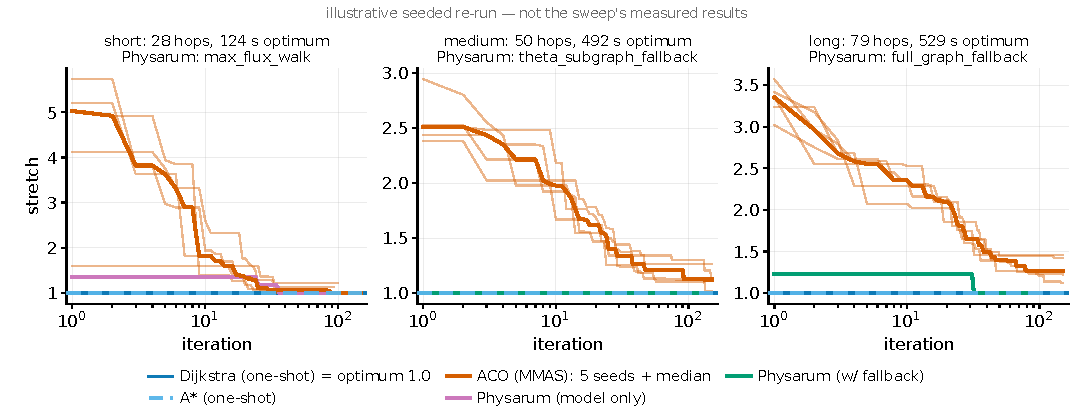
\includegraphics[width=\columnwidth]{fig01_convergence.pdf}
\caption{Cost versus iteration across three distance strata. The Physarum
with-fallback series begins at stretch 1.0 in two of three panels: that is
the fallback, not convergence.}
\label{fig:convergence}
\end{figure}

We therefore report Physarum as two labelled series everywhere below, and
never pool them.

\subsection{Pre-disruption path quality}

Table~\ref{tab:quality} gives the undisrupted comparison. Dijkstra and A*
are exact by construction, and their agreement is the admissibility check of
Section~\ref{sec:algorithms} rather than a result.

\begin{table}[t]
\caption{Pre-disruption path quality, deduplicated on the initial solve.
95\% CIs from the clustered bootstrap.}
\label{tab:quality}
\centering
\small
\begin{tabular}{llrrrr}
\toprule
Series & Traffic & $n$ & Median & Exact & $\leq$10\% \\
\midrule
Dijkstra / A*      & all   & 60  & 1.0000 & 100\%  & 100\% \\
\midrule
ACO (MMAS)         & light & 150 & 1.0052 & 43.3\% & 81.3\% \\
ACO (MMAS)         & heavy & 150 & 1.0209 & 44.0\% & 58.0\% \\
\midrule
Physarum, pooled   & light & 30  & 1.0000 & 86.7\% & 93.3\% \\
Physarum, pooled   & heavy & 30  & 1.0000 & 90.0\% & 93.3\% \\
Physarum, model only & light & 30 & 1.0849 & 16.7\% & 36.7\% \\
Physarum, model only & heavy & 30 & 1.1007 & 23.3\% & 33.3\% \\
\bottomrule
\end{tabular}
\end{table}

ACO's exact-match share is 43--44\% with median stretch 1.005 (light) and
1.021 (heavy). Its per-seed within-10\% spread is tight (0.767--0.833 light,
0.567--0.633 heavy), so this is not a seed artefact. We note separately that
ACO \emph{misses} the exit criterion we set for it in advance --- stretch
$\leq 1.10$ on $\geq 90\%$ of pairs --- reaching 73.3\% under free flow
(95\% CI [58.7, 86.7], the whole interval below the bar) and 80.7\% under
BPR heavy on a held-out pair draw. The failure mode is a colony settling on a
badly wrong corridor and never leaving it: MMAS's own convergence criterion
fires on 79\%/69\% of those solves, so they are settled local optima rather
than unfinished searches. We report this rather than retuning until it
passes.

\subsection{Recovery: warm start buys speed and charges quality}
\label{sec:recovery}

\begin{table}[t]
\caption{Recovery cost, scenarios S1--S6.}
\label{tab:recovery}
\centering
\small
\begin{tabular}{llrrrr}
\toprule
Algorithm & Start & $n$ & Iters & Wall (s) & 1 iter \\
\midrule
Dijkstra  & cold & 358 & 1.0  & 0.031 & 100\% \\
A*        & cold & 358 & 1.0  & 0.027 & 100\% \\
ACO       & warm & 1790 & 69.0 & 34.07 & 0\% \\
ACO       & cold & 1790 & 110.0 & 59.80 & 0\% \\
Physarum  & warm & 358 & 42.0 & 0.235 & \textbf{48.3\%} \\
Physarum  & cold & 358 & 98.0 & 5.661 & 0\% \\
\bottomrule
\end{tabular}
\end{table}

\begin{figure}[t]
\centering
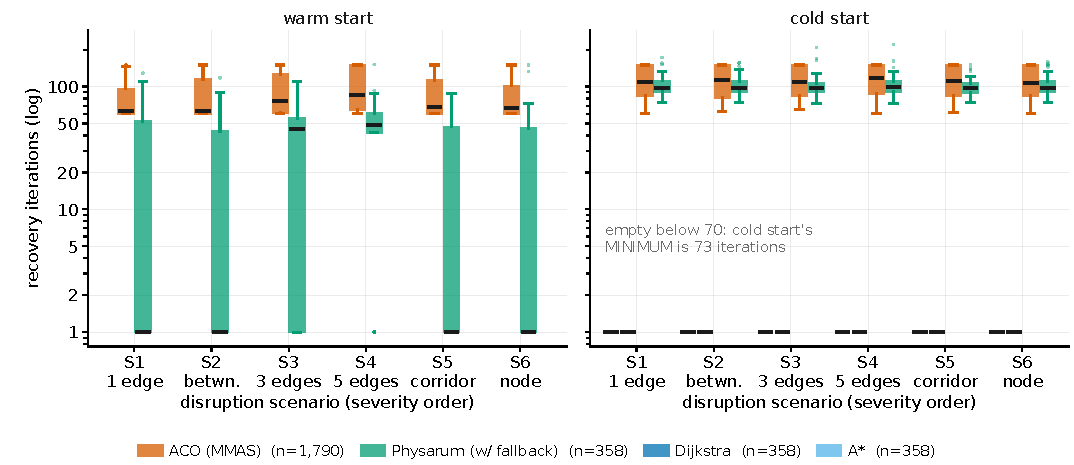
\includegraphics[width=\columnwidth]{fig02_recovery_by_scenario.pdf}
\caption{Recovery iterations by closure severity. Dijkstra and A* collapse to
a line at one iteration. S0 is absent by construction: it has no recovery to
measure, and plotting its nulls as zeros would fabricate a measurement. The
warm panel omits the classical routers, which have no warm mode.}
\label{fig:byscenario}
\end{figure}

\textbf{Dijkstra wins on wall-clock and we report it plainly.} A recompute on
this graph costs about 31\,ms; the bio-inspired methods take seconds. The
interesting quantities are iterations-to-adapt and post-disruption quality.

Paired on identical cells, warm start reduces Physarum's recovery by
\textbf{2.97$\times$ in iterations} (warm faster on 350 of 358,
$p=3.2\times10^{-59}$) and \textbf{6.87$\times$ in wall-clock} (336 of 358,
$p=9.0\times10^{-52}$). For ACO the gains are smaller but significant:
1.26$\times$ and 1.56$\times$ ($n=1{,}790$, $p=1.5\times10^{-184}$).

Two observations matter more than the ratios. First, \textbf{the
distribution is bimodal, not merely shifted}: 48.3\% of warm recoveries
converge in exactly one iteration, while cold start never does and its
minimum is 73 (Fig.~\ref{fig:warmcold}). The retained field already encodes a
viable detour, so a single adaptation step suffices. The ratio of the two
medians is not a valid statistic here, and an earlier version of this
analysis that computed one produced a spurious 24$\times$.

Second, \textbf{per-iteration cost is essentially identical} warm versus cold
(0.0511 versus 0.0538\,s), which is what establishes that the saving is
fewer iterations rather than cheaper ones --- the precise claim the
self-healing framing makes.

\begin{figure}[t]
\centering
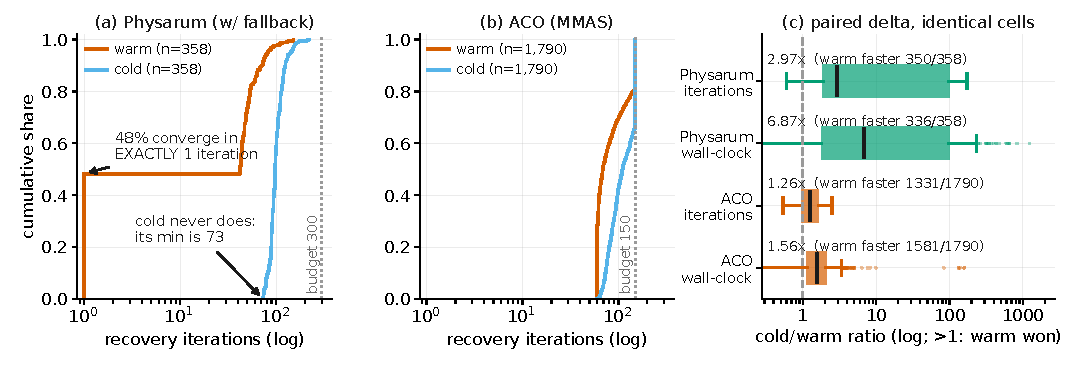
\includegraphics[width=\columnwidth]{fig07_warm_vs_cold.pdf}
\caption{Warm versus cold recovery. The bimodality --- a mode at exactly one
iteration and another near 50 --- is the shape of the result, and is why we
report paired ratios rather than a ratio of medians.}
\label{fig:warmcold}
\end{figure}

\subsubsection{What warm start costs}

Warm start is \emph{not} free, and the cost appears in two places.

On the \textbf{reported path}, paired across all 358 recovery cells, cold
start is better: cold wins on 57 cells, warm on 11, with 290 ties
($p=4.3\times10^{-7}$; mean 1.0669 versus 1.0311, exact match 282 versus
315). On the \textbf{model's own extraction}, the warm maximum-flux walk
completes a path on only 36.3\% of recoveries against cold's 59.5\%.

\begin{figure}[t]
\centering
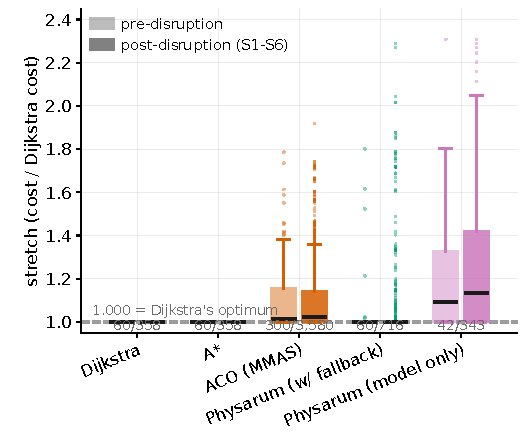
\includegraphics[width=\columnwidth]{fig03_stretch_pre_post.pdf}
\caption{Path quality before and after a closure. Counts beneath each pair are
$n$(pre)\,/\,$n$(post). The two Physarum series are never pooled: the
model-only series is null --- not zero --- on runs where the walk never
completed a path, so its $n$ is smaller by construction.}
\label{fig:prepost}
\end{figure}

An earlier version of this analysis compared the walk's quality unpaired,
across samples of different size, and reported the opposite sign. On the 126
cells where both complete, cold's walk appeared marginally better (1.0127
versus 1.0587, $p=2.7\times10^{-4}$) --- but Section~\ref{sec:adaptation}
shows that this advantage is bought at iteration one by a field that has not
yet run the model, and that at the final iteration the two modes are
statistically indistinguishable.

\subsubsection{Why warm start hurts the walk}

We tested the obvious explanation --- that a retained field keeps driving
flux down now-severed corridors --- and \textbf{refuted it}. A placebo
closure placed at least eight hops from every node of the retained corridor
reproduces almost the entire deficit (warm 43.3\% versus cold 70.0\%,
$n=60$, $p=3.1\times10^{-5}$), and placebo versus a closure sitting directly
on the route is \emph{indistinguishable} (43.3\% versus 41.7\%, $n=60$
paired, $p=1.00$). Spatial locality is flat: the warm walk's terminal node
lies a median 12 hops from the nearest closed edge, and so does cold's
($p=0.356$).

A second candidate --- that warm start simply leaves less conductivity ---
is \emph{analytically impossible}. Scaling $D$ by $c$ scales $w = D/L$ by $c$
and hence $p$ by $1/c$, leaving $Q = w\,\Delta p$ exactly unchanged. We
verified this numerically: rescaling by $10^{-3}$ and $10^{3}$ changes the
flux by less than $10^{-15}$. Only the \emph{shape} of the field can matter,
never its level.

What the data support is this: \textbf{the maximum-flux walk works on a
near-uniform field and stops working as the field converges onto a thin
corridor.} Whether the walk completes on the final pre-disruption iteration,
with the graph fully intact, predicts warm recovery completion on 314 of 358
cells (87.7\%, Fisher $p=1.4\times10^{-50}$). Convergence alone, with no
closure anywhere, drops completion from 69.8\% to 43.0\%. Cold start's
advantage is not that it explores more freely relative to the closure --- it
is that it \emph{rewinds the field to the uniform state the walk can
traverse}.

\begin{figure}[t]
\centering
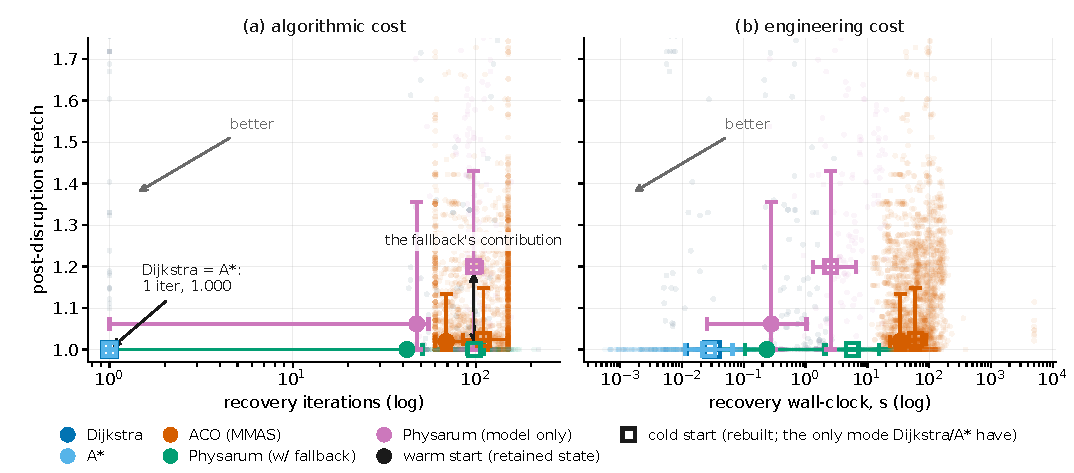
\includegraphics[width=\columnwidth]{fig04_pareto_recovery_vs_quality.pdf}
\caption{The speed-versus-quality trade, and the direct answer to the
question this paper asks. One marker per series and start mode at the median,
with IQR arms on both axes, over a scatter of individual S1--S6 recovery
runs. Dijkstra and A* anchor the lower left: exact paths in one iteration and
roughly 30\,ms. The model-only Physarum series uses the same runs as the
pooled one, so its $x$ is identical and only its $y$ differs --- \emph{the
vertical gap between the two Physarum markers is the fallback's
contribution}.}
\label{fig:pareto}
\end{figure}

\subsection{What adaptation actually contributes}
\label{sec:adaptation}

The preceding result invites the conclusion that convergence is a liability
and that the model should stop earlier. We tested that directly against a
zero-adaptation control: the same pressure solve on a uniform conductivity
field, which is an electrical flow on a travel-time-resistive network
containing none of the Tero dynamics. The control is exact by construction,
since the solver computes pressures and extracts before updating $D$, so its
first iteration \emph{is} the unadapted field.

\begin{table}[t]
\caption{Zero-adaptation control versus the converged field, 60 undisrupted
solves.}
\label{tab:adaptation}
\centering
\begin{tabular}{lrr}
\toprule
 & Uniform (no adaptation) & Converged \\
\midrule
Walk completes      & \textbf{0.567} & 0.433 \\
Walk stretch, median & 1.4367 & \textbf{1.0059} \\
Exact $\mid$ completion & 5.9\% & \textbf{46.2\%} \\
\bottomrule
\end{tabular}
\end{table}

\textbf{Completion and quality move in opposite directions.} The unadapted
field reaches the target more often and produces routes more than 40\% above
optimal; the converged field reaches it less often and is near-optimal when
it does. Paired on the same solves, the unadapted field loses 26--0 to the
best adapted iteration ($n=34$, $p=8.3\times10^{-6}$) and 15--3 to the final
iteration ($n=21$, $p=0.0156$); this reproduces at scale on cold recovery
(120--1, $n=176$, $p=3.2\times10^{-21}$) and warm (27--5, $n=82$,
$p=1.0\times10^{-3}$).

The mechanism is that a near-uniform field is walkable \emph{because} it is
uninformative: flux spreads across many routes, so almost every node has a
positive-flux successor, and the route strung together is poor. This also
resolves the apparent conflict with~\cite{wang2021transition}: their claim
that the dominant path at convergence is the shortest path is about quality,
and on our substrate quality indeed improves with convergence --- what fails
is \emph{completion}, which a complete graph cannot exhibit.

\textbf{No earlier stopping rule is worth adopting.} No fixed iteration count
beats the $\max|\Delta D| < \epsilon$ criterion in any of our three
censuses. A perfect per-cell oracle buys \emph{zero} additional exact
matches, because every exact-match walk is already exact at the final
iteration; it adds only 16 completions of mediocre paths (median stretch
1.2479, none optimal), moving the within-10\% rate from 0.267 to 0.350.
Moreover the walk's best iteration is dispersed (median 26.5, IQR
12.25--33.5), so no fixed rule could capture it, and the router already
retains the best walk across all iterations --- so there is nothing to gain
by stopping at all.

\subsection{The congestion model determines the sign of the effect}

On the undisrupted solve, ACO's within-10\% rate is 81.3\% under light SUMO
demand and 58.0\% under heavy, and paired on the same (OD, seed) cells heavy
is significantly worse ($p=0.036$; 37 pairs pass only under light against 2
only under heavy).

This \emph{reverses} what we measured on the analytic BPR provider, where
congestion improved ACO's outcomes because it flattens the cost surface and
more routes land within 10\% of optimal. The algorithm, the network and the
OD pairs are identical; only the congestion source differs.

\textbf{The sign of the congestion effect is therefore a property of the
congestion model, not of the algorithm}, which is direct evidence for the
bracketing warning of Section~\ref{sec:network}. We draw a methodological
conclusion from it: any claim about routing behaviour ``under congestion''
that does not name its congestion model is underdetermined. We accordingly
retract a framing from our own earlier analysis --- that the two
bio-inspired methods fail in opposite directions under congestion --- which
held on BPR and does not survive SUMO, where both degrade.

\subsection{Network fragility is super-additive}
\label{sec:fragility}

The rejection rates in Table~\ref{tab:scenarios} are a measurement of the
network rather than of the algorithms, taken over 4{,}200 disruption
generations with zero infeasible outcomes.

The network is \textbf{not} fragile to single closures: only about one path
edge in 40 is a cut edge for its own OD pair, as expected of a dense
irregular grid. But fragility is \textbf{super-additive} in simultaneous
closures --- 2.6\%, 14.5\%, 31.7\% for one, three and five path edges, far
faster than linear growth. And a whole closed \emph{corridor} is
\emph{safer} than five scattered edges (7.4\% at a median of four and up to
60 edges, against 31.7\% at five), because corridor edges are consecutive, so
a single detour routes around all of them. Congestion moves none of this by
more than about one percentage point, as expected, since connectivity is
topological.

\section{Discussion}

\subsection{Why a real road network was necessary}

Each of our main findings is invisible on the graph families that dominate
this literature, and for a structural reason rather than a matter of scale.

The maximum-flux walk fails by \emph{dead-ending}: it reaches a node with no
admissible unvisited successor. On a complete graph that is impossible, since
every unvisited node is adjacent; on a small-world graph of mean degree 6 to
600 it is vanishingly rare. Our network has mean out-degree 2.46, and the
undirected pressure solve routinely prefers a direction the road forbids. The
failure mode we spent most of this study measuring is structurally
unreachable on the substrates where the model's accuracy was established.

This reframes the disagreement with prior work as a question of domain rather
than of correctness. Zhang et al.\ report 100\% accuracy with \emph{no}
extraction machinery at all~\cite{zhang2014improved}, and they are entitled
to: on Erd\H{o}s--R\'enyi graphs the flux separates cleanly and reading the
path off is trivial. Wang et al.\ state that the dominant path at
convergence \emph{is} the shortest path~\cite{wang2021transition}, on
explicitly undirected graphs where the walk cannot dead-end. Neither result
is wrong. What changes on a directed, sparse, organically grown network is
that extraction stops being a formality and becomes the step that determines
the reported outcome.

\subsection{Provenance as a reporting requirement}

The practical consequence is a reporting rule. A Physarum accuracy figure on
a network of this kind is a statement about the extraction policy at least as
much as about the model, and a pooled number is unfalsifiable: our own
pooled 90\% and model-only 23.3\% come from the same solves. We would argue
that any Physarum evaluation on a directed network should publish the
provenance distribution of its reported paths, and that a model whose
fallback is a shortest-path algorithm must report what share of its results
that fallback produced.

The warm-start case shows how far this can go. At 66.8\% full-graph fallback,
a warm Physarum recovery is more likely to be Dijkstra's answer than the
model's, and an evaluation reporting only pooled stretch would record that
configuration as near-perfect. It was precisely such a configuration --- the
stranded-component degeneracy of Section~\ref{sec:algorithms} --- that
produced a fabricated mean stretch of exactly 1.000 on the scenario where
the model is weakest, with no error raised. Instrumenting provenance is what
made that visible.

\subsection{What self-healing is actually worth here}

Our answer to the motivating question is a quantified trade rather than an
endorsement or a dismissal.

The adaptive state is real and it is substantial: warm start recovers in a
single iteration on nearly half of all closures, which cold start never
achieves, and per-iteration cost is unchanged, so the saving is genuinely
adaptation. That is the strongest form of the self-healing claim we can
support, and it is stronger than any ratio we could quote.

But it is paid for. Warm start is significantly worse on the reported
post-disruption path, and it degrades the model's own extraction further
still. A system that must guarantee route quality after a closure should
prefer a cold solve or a recompute; one that must respond within a single
adaptation step, and can tolerate a few percent of path cost, is the case
where retained state pays. Neither conclusion is available from the speed
measurement alone.

Against all of this stands the baseline. Dijkstra recomputes an exact route
in about 31\,ms on this network, and none of the bio-inspired methods comes
close on wall-clock. For a graph of a few thousand nodes, recomputation is
simply the right engineering answer, and the interest in these methods has to
rest on regimes we did not test --- far larger networks, many simultaneous
commodities, or settings where the cost function is not globally observable.
We think it is more useful to say so than to construct a comparison the
baseline would lose.

\subsection{A methodological result about benchmarking}

The congestion-model finding generalises beyond this study. We measured
opposite signs for the effect of congestion on ACO from an analytic
volume-delay function and from a microsimulator, on the same network with the
same OD pairs. Both are standard and defensible choices; they differ because
SUMO puts signal delay in the numerator but not the free-flow denominator,
while BPR loads synthetic demand onto shortest paths, which is exactly where
an OD-path measurement walks.

A benchmark that reports results ``under congestion'' without naming the
source is therefore not reproducible in the sense that matters, because an
equally reasonable alternative can reverse the sign of its headline effect.
We would encourage reporting both where feasible, treating them as brackets
rather than as substitutes, and never merging them into a single congestion
level.

\section{Threats to Validity and Limitations}
\label{sec:limitations}

\subsection{Scope of the measurement}

\textbf{One city, one bounding box.} All results are from a single
$\sim$4$\times$4\,km area. The structural properties we argue are decisive
--- low out-degree, pervasive one-ways --- are common to dense organically
grown cities, but we have not demonstrated that the findings transfer, and a
grid-planned city could behave differently precisely because its out-degree
is higher and more uniform.

\textbf{Synthetic demand.} Our congestion comes from simulated demand rather
than calibrated traffic counts. This is the dimension on which the closest
recent ACO work is stronger: Tuan et al.\ use measured loop-detector
speeds~\cite{tuan2026improved,li2018diffusion}. We traded measured demand for
a controlled, repeatable closure protocol over a full directed street
network, which their dataset does not support; the complementary study is
worth doing.

\textbf{Absolute times are optimistic.} Because the shared baseline
re-annotates free-flow speeds from the generated network, mean free-flow
speed is considerably higher than real Bengaluru conditions. Every quantity
we report is a ratio or a count for this reason. Absolute seconds in this
paper should not be read as travel-time predictions.

\textbf{Single-commodity Physarum.} We run one Physarum instance per OD pair
rather than modelling multi-commodity flow. This matches the model's
single-source/single-sink formulation and the comparison we wanted, but it
forgoes the network-formation behaviour that motivates much of the Physarum
literature~\cite{tero2010rules}.

\subsection{Choices that could have gone otherwise}

\textbf{We did not implement the directed Physarum formulation.} A directed
variant exists~\cite{zhang2014directed}. We deliberately benchmarked the
canonical model, since that is what the accuracy claims in the literature
describe, but our extraction findings should be read as characterising the
canonical model on a directed network --- an acknowledged limitation of that
model --- rather than as a statement about what Physarum-style methods can
achieve in principle.

\textbf{The dead-node memo is lossy.} About 66\% of its prunes refuse a node
that was still viable for the ant in question, and memo-on paths are a strict
subset of memo-off paths. It is a deliberate construction heuristic and the
ACO numbers should be read with it in place.

\textbf{A prefer-walk-on-tie policy was measured but not applied.} Because
the best cost is a strict minimum over iterations, the walk can tie the
fallback and still be scored a loss. Preferring the walk on ties would raise
the free-flow provenance share from about 33\% to roughly 50\% \emph{without
changing a single reported cost}, and would recover nothing under
congestion. We left it out because it changes the semantics of the best-cost
tracker, but it means our model-only shares are mildly conservative under
free flow.

\textbf{ACO's hyperparameters were tuned; Physarum's largely were not.} The
comparison is between a tuned ACO and a near-default Physarum, which is a
real asymmetry. We note in mitigation that Physarum's single seed is
justified by measurement rather than assumption, and that the extraction
findings concern a structural failure mode rather than a parameter setting.

\subsection{Statistical caveats}

The design is fully paired, and the pairing is verified rather than assumed:
pre-disruption walk stretch is byte-identical warm versus cold across 250
cells, as it must be, since before the closure the two modes are the same
run. Where we report conditional statistics --- notably the model-only
median, which exists only where the walk completed --- the denominator
differs from the unconditional shares, and reading one as the other would
mislead. Two errors of exactly this kind occurred during the work and were
corrected; we have stated both in Section~\ref{sec:design} because they are
easy to repeat.

Finally, the literature search supporting our novelty claim covers the open
citation databases and complete forward-citation sets for the two most likely
anchor papers, but not the IEEE Xplore and Scopus native interfaces, Google
Scholar's full-text index, or venues that index poorly. Two full texts were
judged from their abstracts. We regard the claim as systematically supported
for the indexed literature rather than exhaustively verified.

\section{Conclusion}

We benchmarked classical, ant-colony and Physarum routing on the real
directed road network of central Bengaluru under microsimulated congestion,
measuring recovery from seven classes of road closure as well as path
quality, over 5{,}520 runs in a fully paired design.

The headline claim made for bio-inspired routing --- that retained internal
state buys recovery without recomputation --- holds, and holds in its
strongest form: warm start lets Physarum recover in a single iteration on
48.3\% of closures, which cold start never achieves, at an unchanged
per-iteration cost. But it is a trade and not a gift. Warm start is
significantly worse on the reported post-disruption path, and it degrades the
model's own extraction further, so reporting only the speed-up describes half
the effect.

The finding we think matters most is methodological. A Physarum model does
not emit a route; an extraction step does, and on a sparse directed network
that step decides the answer. Pooled over extraction methods our Physarum
matches the optimum on 90\% of undisrupted pairs; using only its own
maximum-flux walk, 23.3\%; and on warm recoveries it returns plain
Dijkstra's path two-thirds of the time. Because the median stretch is
exactly 1.000 inside every provenance class, a pooled figure cannot be
falsified. We argue that provenance should be reported as a matter of course
for this model class.

We also showed that adaptation improves extraction \emph{quality} while
reducing its \emph{reliability}, so the two must be measured together; that
no earlier stopping rule improves on the standard convergence criterion,
because the quality ceiling is already reached there; and that the sign of
the congestion effect on ACO belongs to the congestion model rather than to
the algorithm, which makes unqualified claims about behaviour ``under
congestion'' underdetermined.

Throughout, Dijkstra remained the honest baseline: an exact route in one
iteration and roughly 31\,ms, which no method here approached on wall-clock.
On a network of this size recomputation is the correct engineering choice,
and the case for adaptive methods must be made on regimes we did not test.

Future work should extend the benchmark across cities with different
topological character, pair the controlled closure protocol used here with
measured rather than synthetic demand, and evaluate the directed Physarum
formulation, whose behaviour on this substrate our results give specific
reason to want measured.

\section*{Reproducibility}

The complete experimental record --- the 5{,}520-row results file from which
every number in this paper derives, the network and congestion pipeline, all
seven figure-generating scripts, the hyperparameter sweeps, and the
pre-registered measurement protocols for the mechanism experiments --- is
available in the project repository. Every run carries its seed and a
configuration hash, and all figures regenerate from the committed results
file with a single command. Recorded failures are retained rather than
dropped, and a deliberately failing test marks the ACO exit criterion that
was missed.


\bibliographystyle{IEEEtran}
\bibliography{refs}

\end{document}
